\chapter{Implémentation}
\label{ch:implémentation}

\section{L'API WiFace}

\subsection{Choix de la stack}

Du côté serveur, le langage utilisé est le Python (3.7). Pour faciliter le développement d’une API rest, le micro-
framework \textbf{Flask} a été choisi. Au vu de la documentation et de mon expérience personnelle, ce choix est pertinent
dans le cadre de ce projet.

Avantages de Flask :
\begin{itemize}
\item Simple et léger
\item Convient bien au développement d’application de petite ou moyenne envergure
\item Très flexible
\item Prise en main rapide
\item Compatible avec l’ORM sqlalchemy
\end{itemize}

L’ORM qui a été choisi pour fonctionner avec Flask est \textbf{SQLAlchemy}. Il existe en effet un module python flask-
sqlalchemy qui rend l’intégration simple.
Les données sont sérialisées à l’aide de \textbf{marshmallow}.
La gestion de l’authentification se fait à l’aide de token JWT et du module correspondant \textbf{flask-jwt-extended}.
La validation des formulaires a été implémentée à l'aide de \textbf{WTForm}.
La spécification est écrite à l’aide de \textbf{swagger} et de \textbf{connexion}, qui propose également une documentation automatique.

\section{Sniffing des adresses MAC}

Le sniffing des adresses MAC se fait à l'aide de Scapy.
Cette librairie permet de traiter programmatiquement les paquets
reçu par notre antenne. 

Voici le worflow, décrivant le sniffing jusqu'à l'envoi 
des entités à l'API WiFace. 

\begin{figure}[H]
	\centering
	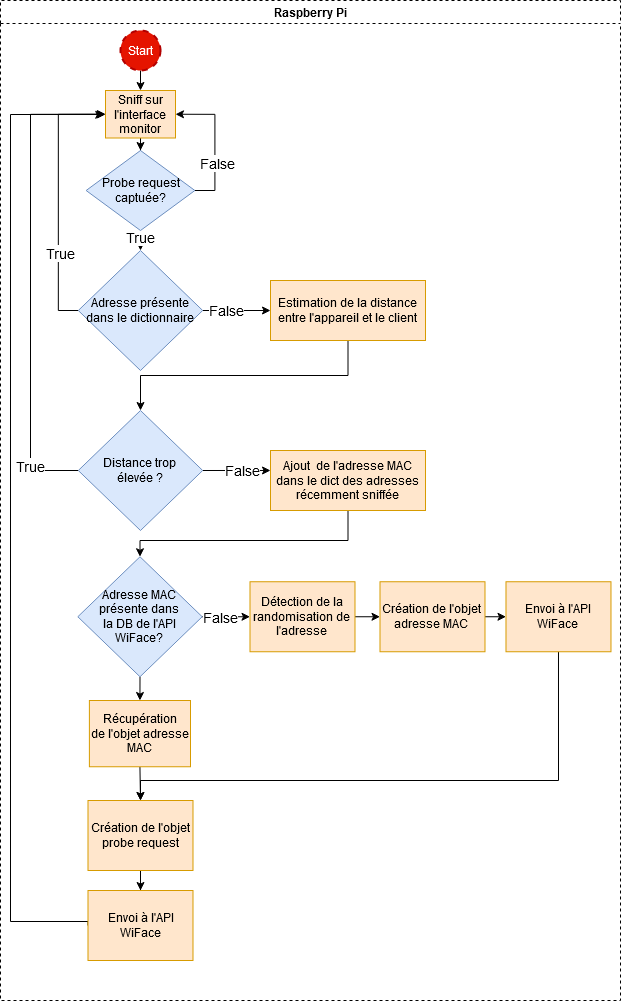
\includegraphics[width=12cm]{images/probe/flowchart_scan_probe.png}
    \caption{Worflow du scan des clients Raspberry}
	\label{fig:worflow-scan}
\end{figure}

Quelques explications concernant les processus de ce diagramme.

\begin{itemize}
    \item \textbf{Sniff sur l'interface monitor}: Dès que scappy reçoit un paquet, un callback est appelé avec ce même paquet en pramaètre.
    \item \textbf{Probe request capturée}: Afin de déterminer si le paquet est bien une probe request, il suffit s'il s'agit d'un paquet 802.11 et d'une trame de management de sous-type 4
    \item \textbf{Adresse présente dans le dictionnaire ?}: Un dictionnaire d'adresse MAC avec le timestamp de capture est maintenu à jour afin de n'envoyer qu'une seule probe request par burst à l'API WiFace.
    \item \textbf{Estimation de la distance}: Une estimation de la distance entre l'appareil et le client est faite à l'aide de la puissance du signal. Cette mesure est très peu fiable et permet seulement de filtrer les probe requests trop lointaines.
    \item \textbf{Adresse MAC présente dans l'API WiFace}: Avant de poster la probe request et l'adresse MAC, il faut d'abord essayer d'obtenir l'ID d'une potentielle adresse MAC déjà existante afin de l'associer à la probe request
    \item \textbf{Détection de la randomisation}: À l'aide de diverses heuristiques (cf \ref{ch:probe_req}) l'adresse est déclarée - ou non - randomisée.
\end{itemize}

\section{La reconnaissance faciale et attribution des identitiés}

La reconnaissance faciale a été implémentée à l'aide d'OpenCV (sur le client Raspberry Pi), de l'API AWS Rekognition et de l'API WiFace
afin de faire le lien entre les deux autres éléments. 

\subsection{Première version du workflow de reconnaissance}

La figure~\ref{fig:worflow-reco} présente le worflow permettant, depuis une image capturée par la PiCamera, d'attribuer une identité et diverses propriétés.

\clearpage
\newpage

\thispagestyle{empty}
\begin{landscape}
    \centering
\thispagestyle{empty}
\begin{figure}[ht]
     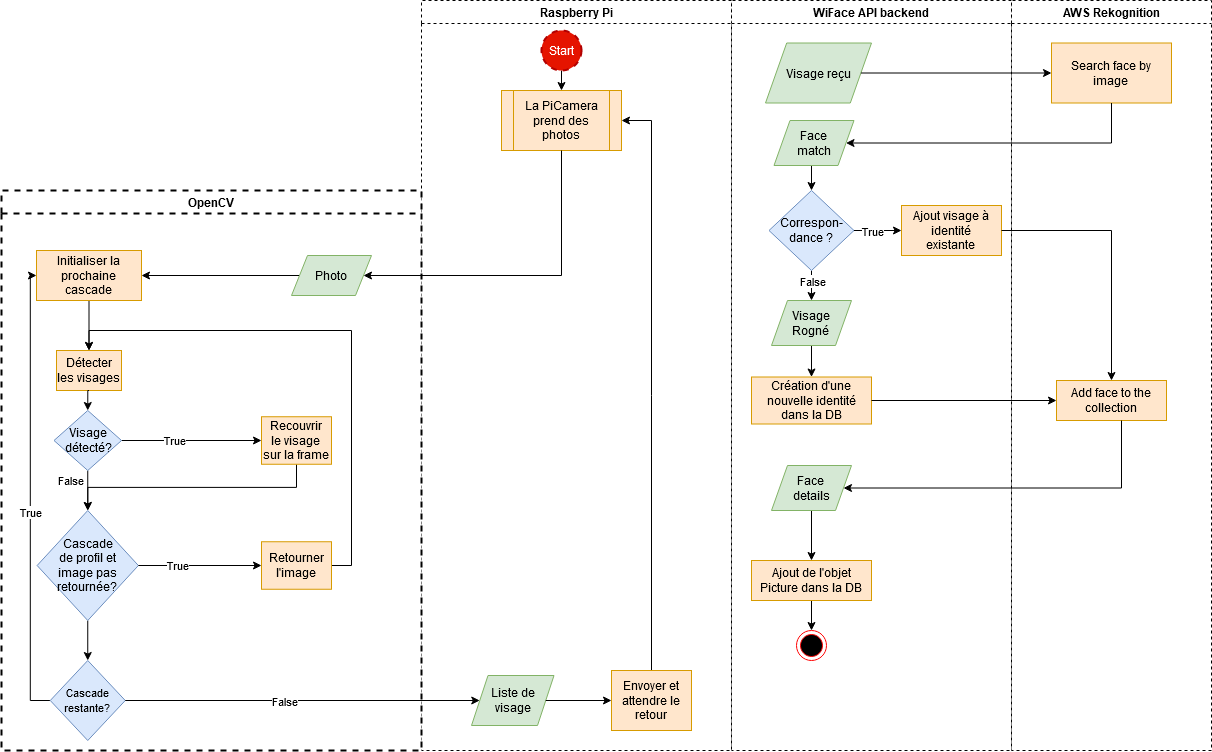
\includegraphics[width=0.95\linewidth]{images/facial_reco/flowchart_reco_v2.png}
     \caption{Worflow de la reconnaissance faciale}
     \label{fig:worflow-reco}
\end{figure}
\end{landscape}

Quelques explications concernant les inputs, outputs et processus de ce diagramme.

Raspberry Pi et OpenCV:
Le but de cette partie est de filter les images intéressantes (contenant un visage). En effet,
cela permet de ne pas avoir à envoyer des milliers d'images à l'API d'Amazon qui possède un quota.
\begin{itemize}
    \item \textbf{La PiCamera prend des photos} en boucle tant que le programme est en activité et qu'une reconnaissance n'est pas en cours.
    \item \textbf{Initialiser la prochaine cascade}: Les cascades de Haar d'OpenCV ont été utilisée. Les pertinentes sont celles pré-entraînée pour de la reconnaissance frontale et de profil.
    \item \textbf{Détecter les visages}: Les visages sont détectés grâce à la fonction \textbf{detectMultiScale} qui renvoie les coordonnées de chaque visage détecté.
    \item \textbf{Cascade de profil et image pas retournée?}: Condition qui exprime si la cascade actuelle est celle qui détecte les visages de profil, et si l'image n'a pas déjà été retournée.
    \item \textbf{Retourner l'image}: Consiste à faire une symétrie axiale en Y de l'image. Les cascades d'OpenCV sont entraînées pour un seul des deux profils. Nous maximisons les chances de détection ainsi
    \item \textbf{Recouvrir le visage sur la frame}: Afin de ne pas redétecter les mêmes visages avec les prochaines cascades, nous utilisons les coordonnées obtenus et remplaçons le visage par un rectange sur la frame original, le visage est sauvegardé avant.
\end{itemize}

WiFace API et Amazon rekognition:
L'API WiFace reçoit alors les images rognées de visage. 
C'est elle qui va communiquer avec Rekognition et mettre à jour la base de donnée.
Rekognition se chargera d'éliminer les faux-positifs d'OpenCV et de faire la vraie reconnaissance de visage,
afin de savoir si ce dernier se trouve dans notre collection.
\begin{itemize}
    \item \textbf{Search face by image}~\ref{text:SearchFacesByImage}
    \item \textbf{Correspondance ?}: Selon la réponse de Rekognition, deux scénarios existent. Si le visage a été reconnu, il faut associer l'image à l'identité existante, sinon en créer une nouvelle.
    \item \textbf{Face details}: Cette output de Rekognition contient des données intéressantes que nous allons associer à l'image (et donc à l'identité). Parmi ces données, nous trouvons:
    \begin{itemize}
        \item Le genre (Homme / Femme) du sujet
        \item Une fourchette d'âge probable du sujet
        \item Une liste de plusieurs émotions que le sujet pourrait exprimer (triste, heureux, effrayé..)
        \item La présence, ou non, de certains accessoires ou caractéristiques (lunettes, barbe,..)
    \end{itemize} 
\end{itemize} 

\subsubsection{Problèmes de cette implémentation}\label{sec:probleme_workflow}
Bien que le processus ait été implémenté et est fonctionnel,
quelques problèmes méritent d'être résolu.

En effet, lors de tests, il a été remarqué que la détection d'Amazon
donnait de meilleurs résultats concernant les FaceDetails lorsque l'image d'une personne
était envoyée au complet, au lieu d'être rognée. Il a donc été déduit que le traitement fait par OpenCV engendrait de la perte
d'information pour le modèle d'Amazon.

De plus, effectuer systèmatiquement les recherches et découpes de visages sur la Raspberry Pi pourrait résulter en des problèmes de
performances, notamment pour un micro-ordinateur, autant laisser cette responsabilité à Rekognition. Cela a également comme conséquence de limiter
le traffic HTTP entre les clients et l'API WiFace.

\subsection{Deuxième version du worflow}
Suite à ces deux observations, il a été décidé de revoir le worflow comme le montre la figure~\ref{fig:worflow-reco2}

\clearpage
\newpage

\thispagestyle{empty}
\begin{landscape}
    \centering
\thispagestyle{empty}
\begin{figure}%[htb]
     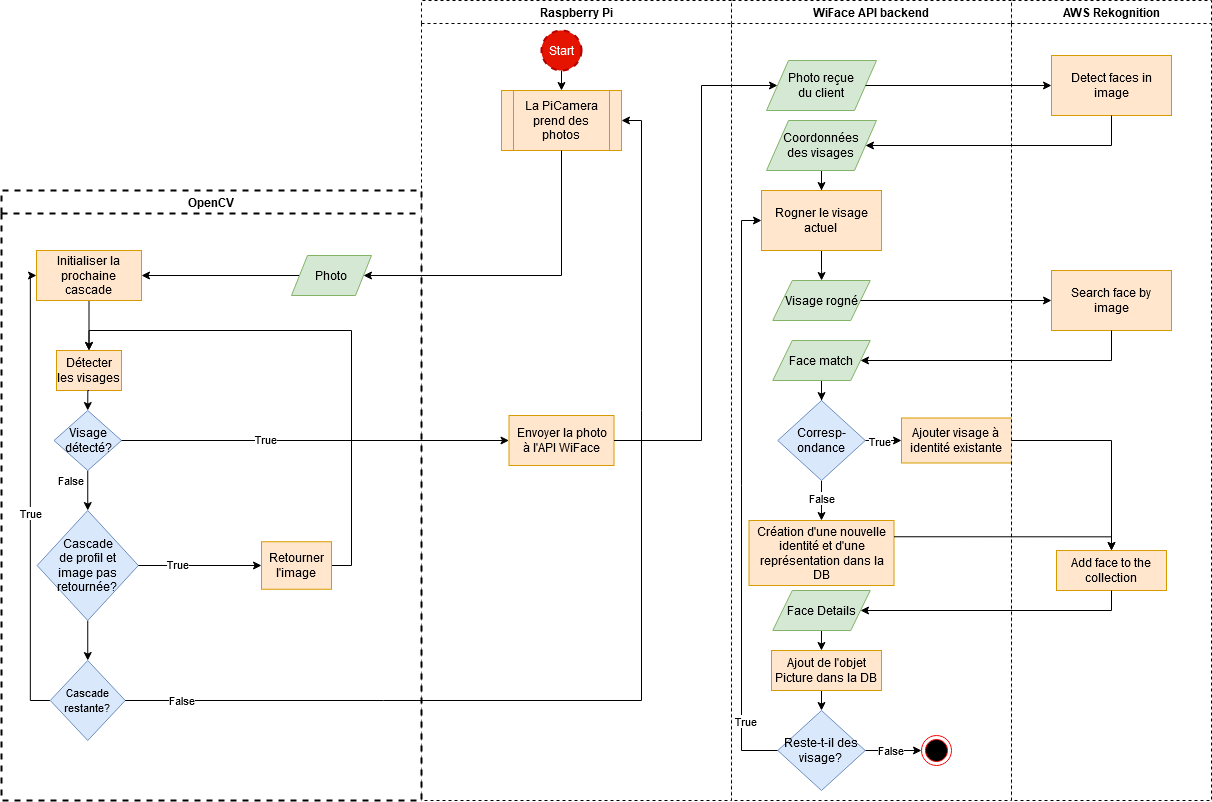
\includegraphics[width=\linewidth]{images/facial_reco/flowchart_reco_v3.png}
     \caption{Deuxième version du worflow de la reconnaissance faciale}
     \label{fig:worflow-reco2}
\end{figure}
\end{landscape}

Les changements suivants ont donc été apportés:
\begin{itemize}
    \item Dès qu'OpenCV détecte un visage, la photo est envoyée en entier à l'API WiFace, sans continuer la recherches
    \item Une nouvelle première étape permet, du côté de Rekognition, de détecter les visages et d'en extraire les coordonnées
    \item L'API WiFace a maintenant la responsabilité de découper les visages et de les envoyer à Rekognition
\end{itemize}

Grâce à ces changements, les problèmes mentionnés dans la section \ref{sec:probleme_workflow} ont été résolus.
\subsection{Exemple du processus}
Voyons avec une image de test (figure~\ref{fig:scott}), comment les différents acteurs de ce Worflow se comportent.
L'image en question comporte deux visages nets, un homme et une femme.

\begin{figure}[H]
	\centering
	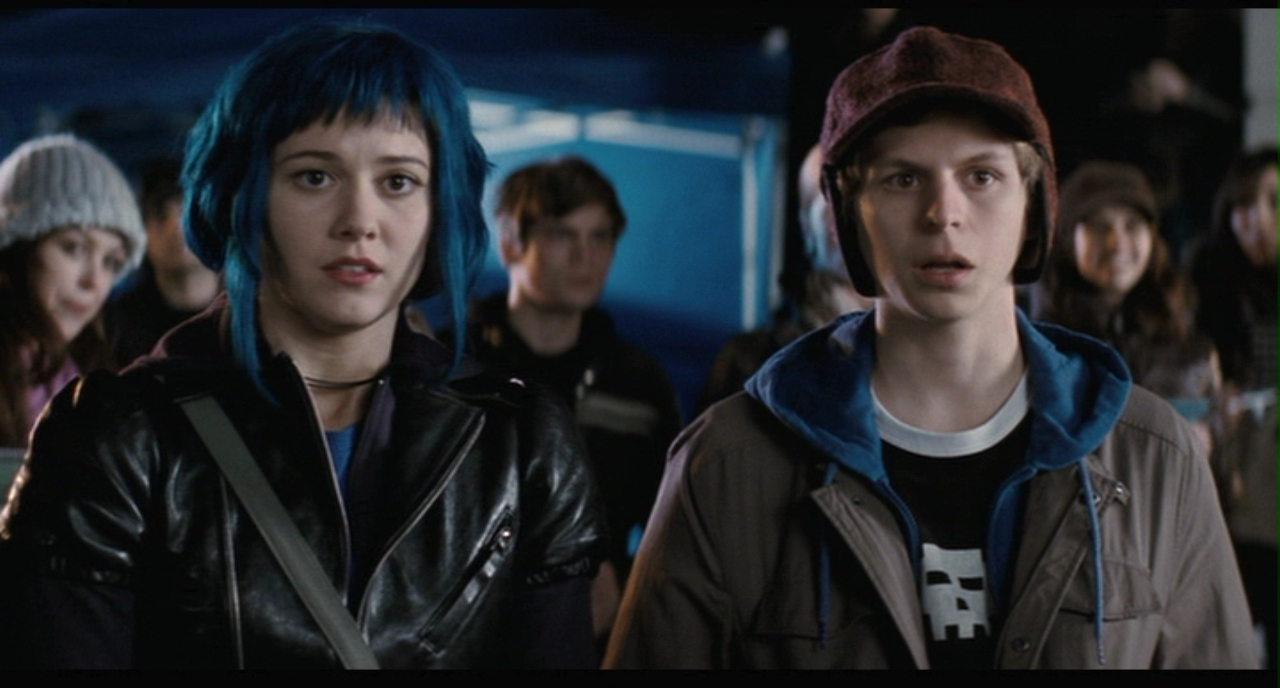
\includegraphics[width=12cm]{images/facial_reco/scott.jpg}
    \caption{Deux visages}
    \source{\cite{SCOTT}}
	\label{fig:scott}
\end{figure}

Cependant, d'autres visages sont aussi présents sur l'image, mais flous. 
Une fois passé au travers d'OpenCV, nous pouvons voir la frame de base recouverte de plusieurs rectangles verts.
Chaque rectangle présent sur la figure~\ref{fig:hidden_face} a été "découpé" et envoyé.

\begin{figure}[H]
	\centering
	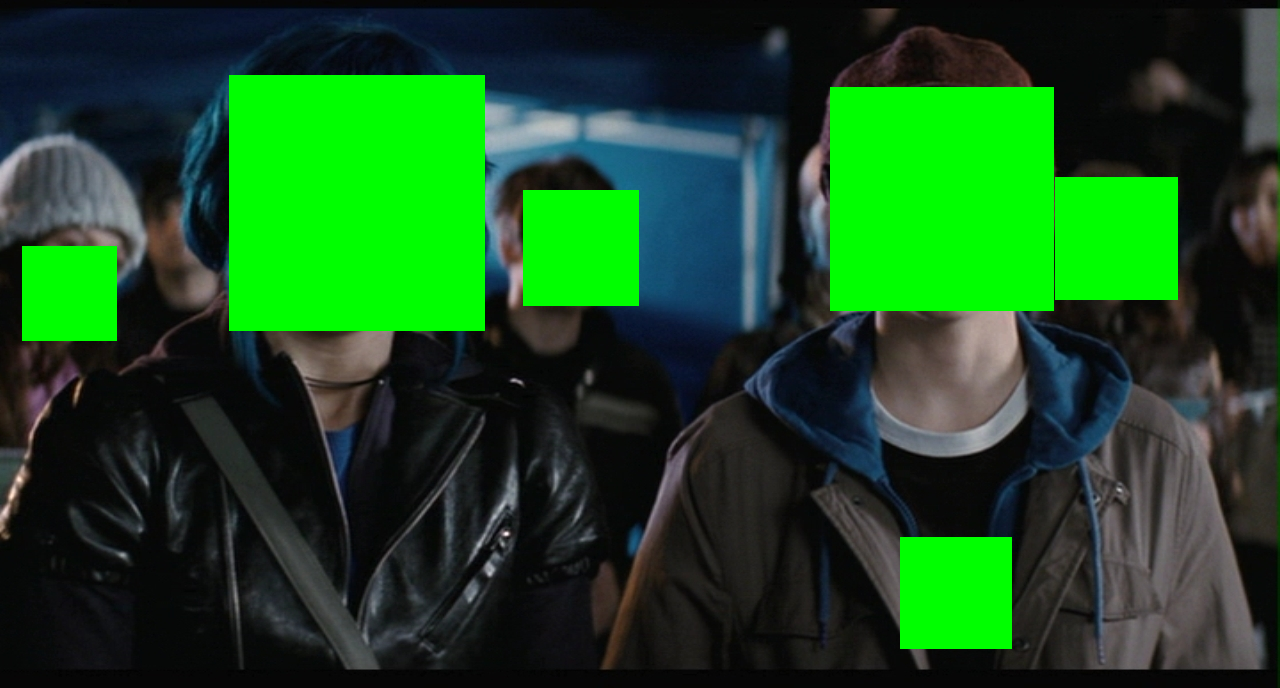
\includegraphics[width=12cm]{images/facial_reco/hidden_face.png}
    \caption{Les visages détectés}
	\label{fig:hidden_face}
\end{figure}

Les deux visages principaux ont été détectés, mais également ceux dans le fond.
Un dessin qui ressemble vaguement à un visage a également été détecté, il s'agit d'un \textbf{faux-positif}.
Cependant, comme Rekognition va à nouveau analyser les images, il est souhaitable qu'OpenCV
soit "trop" sensible, afin de ne pas manquer de potentiels visages.

Les figures~\ref{fig:hidden_face_ramona} et~\ref{fig:hidden_face_scott} montrent les deux visages principaux rognés par OpenCV et envoyé à Rekognition:

\begin{figure}[H]
	\centering
	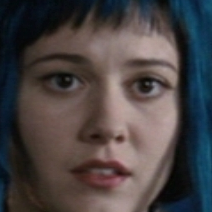
\includegraphics[width=6cm]{images/facial_reco/ramona.png}
    \caption{Visage rogné de Ramona}
	\label{fig:hidden_face_ramona}
\end{figure}

D'après Rekognition:
\begin{itemize}
    \item Genre: Femme
    \item Age: [8 - 18]
    \item Émotion principale: Calme 
\end{itemize}

\begin{figure}[H]
	\centering
	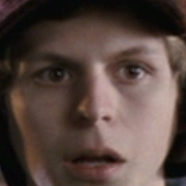
\includegraphics[width=6cm]{images/facial_reco/scott_hidden.png}
    \caption{Visage rogné de Scott}
	\label{fig:hidden_face_scott}
\end{figure}

D'après Rekognition:
\begin{itemize}
    \item Genre: Homme
    \item Age: [14 - 26]
    \item Émotion principale: Confus 
\end{itemize}

Les données reçus sont plutôt correctes, bien que les estimations d'âge soit très vague.

Si nous envoyons une deuxième image (figure~\ref{fig:scott2}), nous voyons alors que les deux sujets ont à nouveau été reconnus, malgré des changements d'apparence (couleur de cheveux).

\begin{figure}[H]
	\centering
	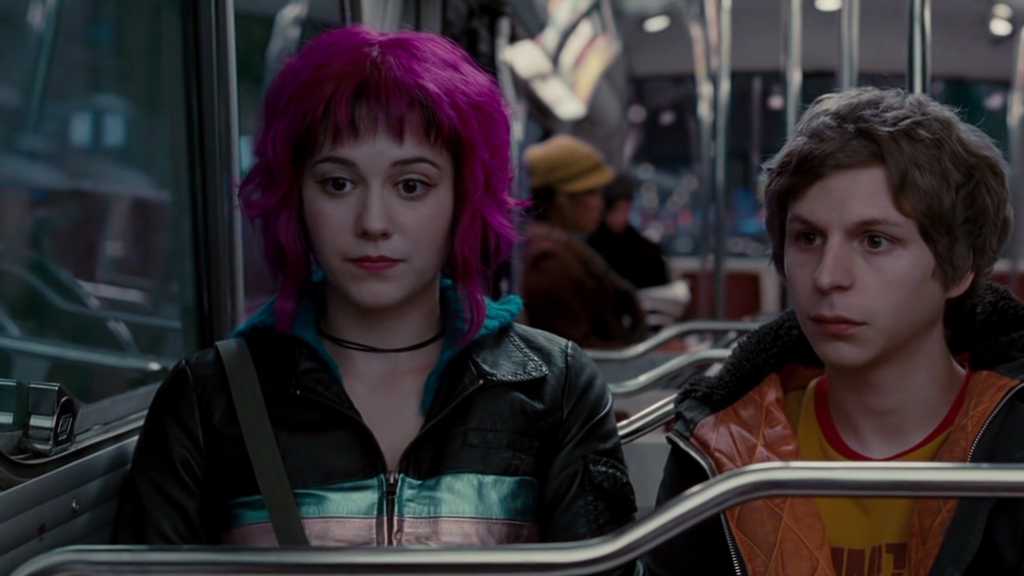
\includegraphics[width=12cm]{images/facial_reco/scott2.png}
    \caption{Deuxième image des sujets}
	\label{fig:scott2}
\end{figure}

La figure ~\ref{fig:ramona_profile} montre le profil de l'identité sur le front-end de WiFace.
\begin{figure}[H]
	\centering
	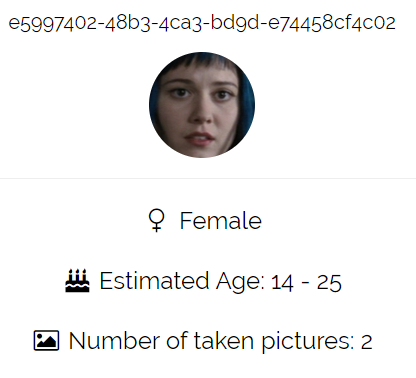
\includegraphics[width=6cm]{images/facial_reco/ramona_profile.png}
    \caption{L'image a été associée au profil existant}
	\label{fig:ramona_profile}
\end{figure}

Les estimations d'âge ont été mises à jour, car il s'agit de la moyenne des données extraites sur toutes les photos d'une identitié.
Le genre est aussi déterminé via la majorité, sur toutes les photos du sujet. 
La photo est séléctionnée comme étant la meilleure (selon les indices de qualité renvoyés par Rekognition)
\section{Le client Raspberry}

\section{Algorithme PP2I}